The "flow past a cylinder" problem consists in a fluid flowing past a cylinder. The problem is a benchmark for the Navier-Stokes equations and a simple example of a flow that gets turbulent with higher values for the Reynolds number.

\subsection{Structure}
In two dimensions, the problem is defined on a rectangular domain with an almost-centered circular obstacle on the left side of the domain, closer to the inflow boundary. For the three dimensional case, the domain is a rectangular prism with a cylindrical obstacle, near the middle of the left side of the domain, similar to the two dimensional case. In fact, the three dimensional case is z-axis extrusion of the two dimensional case, with minor differences in the domain sizes and ratios.

\subsubsection{Boundary conditions}
An homogeneous Dirichlet condition is imposed on both the obstacle and domain boundaries different from the inlet and outlet. In the two dimensional case, the inflow condition is defined as:
\begin{equation}
\begin{cases}
    U(0, y, t) = 4 U_m y (H - y) / H^2 \\
    V = 0
\end{cases}
\end{equation}
Where $U$ and $V$ are the $x$ and $y$ components of the velocity, and $U_m$ is the reference inlet velocity, which can be set through the command line option \texttt{-u}. Alternatively, the inflow condition can be set to be multiplied or not by $\sin(\pi t / 8)$, by using the command line flag \texttt{-v}.

For the three dimensional case, the inflow condition is defined as:
\begin{equation}
\begin{cases}
    U(0, y, z, t) = 16 U_m y z (H - y) (H - z) / H^4 \\
    V = 0 \\
    W = 0
\end{cases}
\end{equation}
Again, interpreting $U$, $V$ and $W$ as the $x$, $y$ and $z$ components of the velocity, with the same support for the command line options \texttt{-u} and \texttt{-v}.

The outflow condition is not defined in the benchmark and was chosen to be a homogeneous Neumann condition, while the initial condition is $\mathbf{u}_0 = \mathbf{0}$.

\subsection{Reynolds number}
The Reynolds number is a central parameter in fluid dynamics, as it can be used to describe the transition from laminar to turbulent flow. The Reynolds number is defined as:
\begin{equation}
    Re = \frac{\bar{U} D}{\nu}
\end{equation}
Where $\bar{U}$ is inlet velocity at a specific point along the inlet boundary, $D$ is the diameter of the cylinder and $\nu$ is the kinematic viscosity of the fluid. The Reynolds number is a dimensionless quantity. For low values of the Reynolds number, the flow is laminar, while for high values, the flow is turbulent.

\subsection{Results}
Figure \ref{fig:velocity-pressure-2d} shows the velocity and pressure fields for different values of the Reynolds number in the two dimensional case and with a constant inlet velocity. Namely, the Reynolds number is 20, 48, 100 and 200, from top to bottom. The velocity field is represented by its magnitude, while the pressure field is represented by its value. Bright, warm colours indicate high values for the relative area. Figure \ref{fig:velocity-3d} shows similar results for the three dimensional case, for $Re = 13, 133$.

\begin{figure}[h]
  \begin{minipage}{\linewidth}
  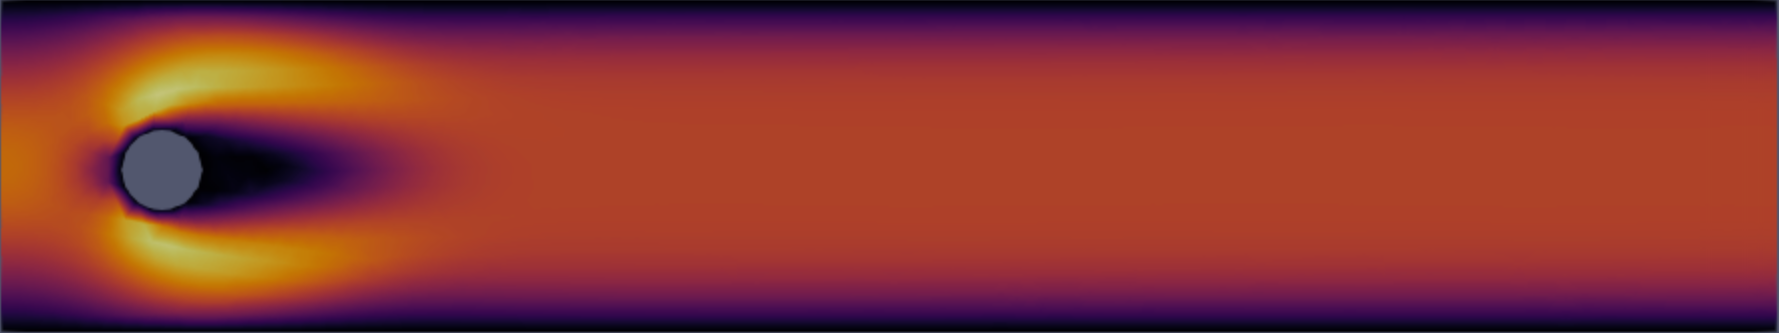
\includegraphics[width=.48\linewidth]{image/velocity-20-2d.png}\hfill
  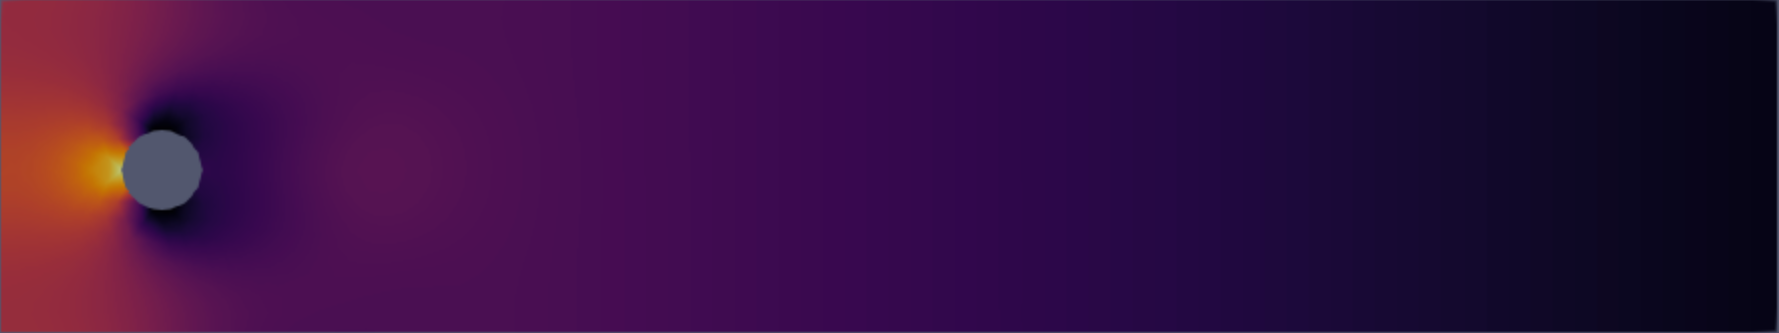
\includegraphics[width=.48\linewidth]{image/pressure-20-2d.png}\hfill
  \end{minipage}%
  \par
  \begin{minipage}{\linewidth}
  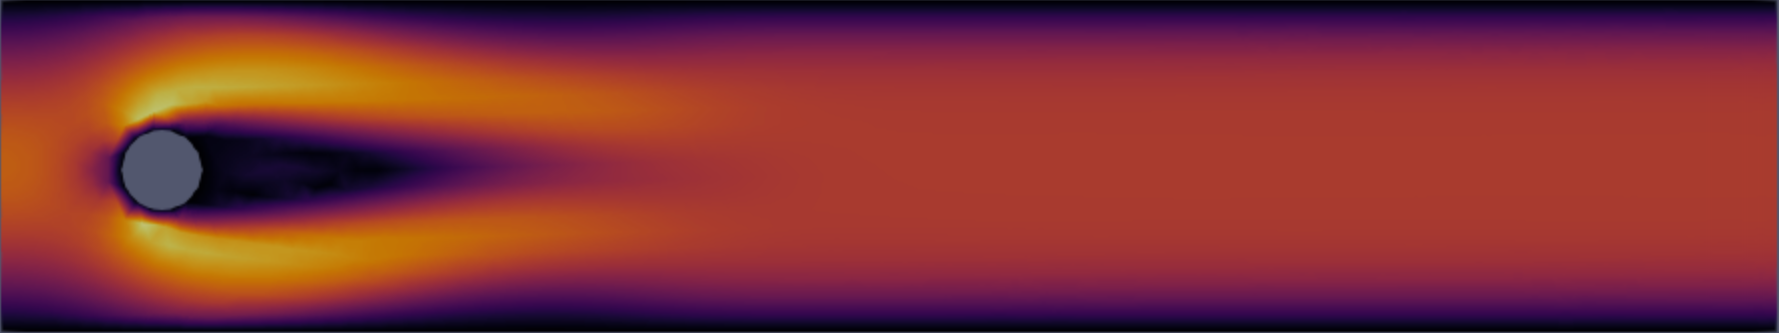
\includegraphics[width=.48\linewidth]{image/velocity-48-2d.png}\hfill
  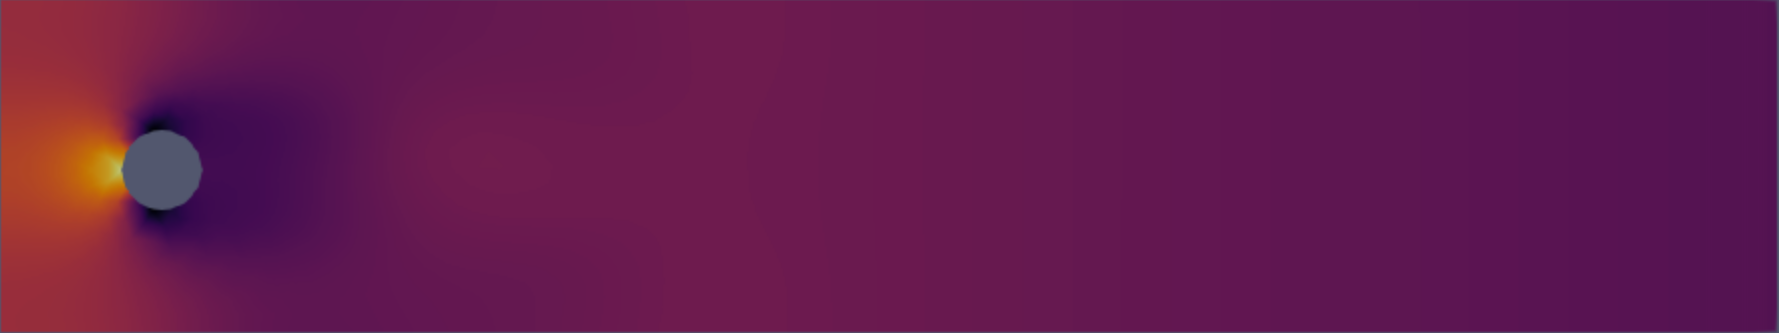
\includegraphics[width=.48\linewidth]{image/pressure-48-2d.png}\hfill
  \end{minipage}%
  \par
  \begin{minipage}{\linewidth}
  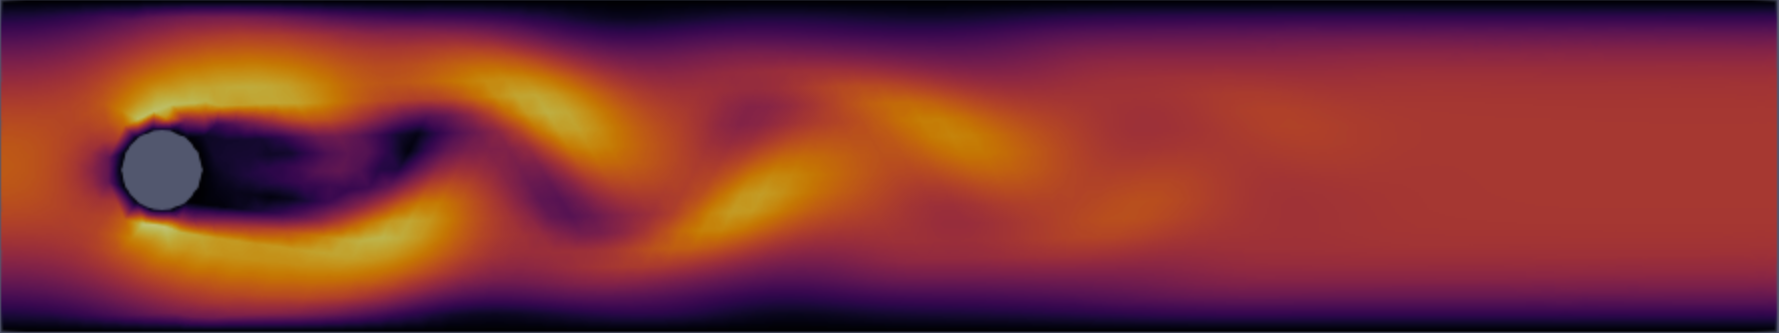
\includegraphics[width=.48\linewidth]{image/velocity-100-2d.png}\hfill
  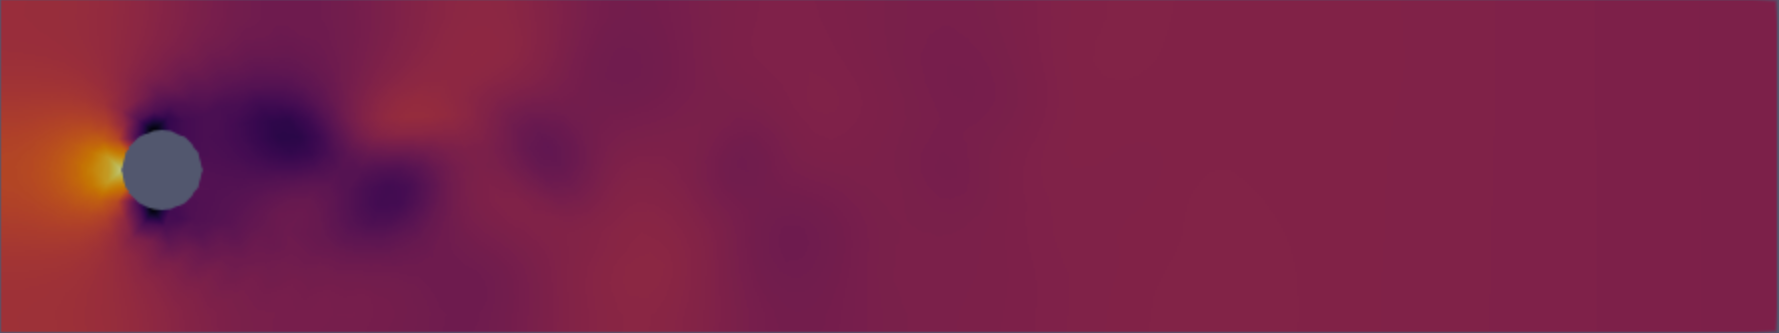
\includegraphics[width=.48\linewidth]{image/pressure-100-2d.png}\hfill
  \end{minipage}%
  \par
  \begin{minipage}{\linewidth}
  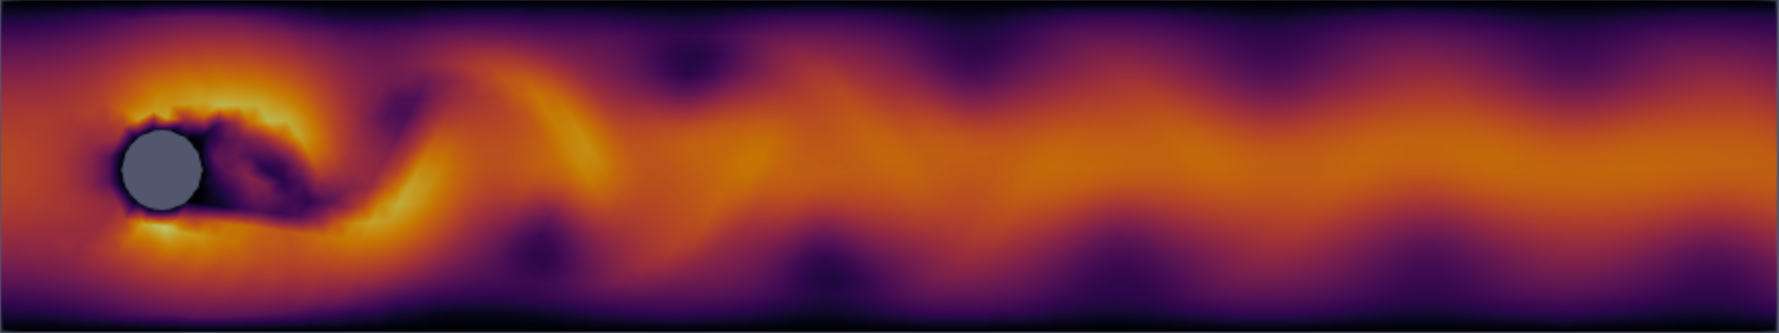
\includegraphics[width=.48\linewidth]{image/velocity-200-2d.png}\hfill
  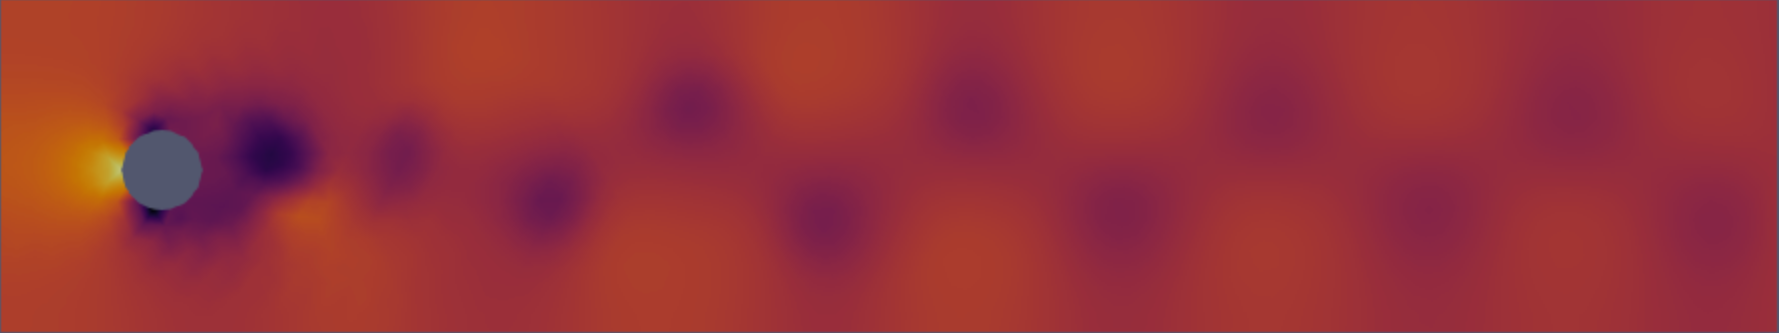
\includegraphics[width=.48\linewidth]{image/pressure-200-2d.png}\hfill
  \end{minipage}%
  
  \caption{Velocity (left) and pressure (right) at different levels of turbulence. The results were obtained with $\Delta t = 5 * 10^{-4}s$, on a mesh generated with the argument \texttt{-clmax 0.25} and are relative to $t = 1.35s$.}
  \label{fig:velocity-pressure-2d}
\end{figure}

\begin{figure}[h]
  \begin{minipage}{\linewidth}
  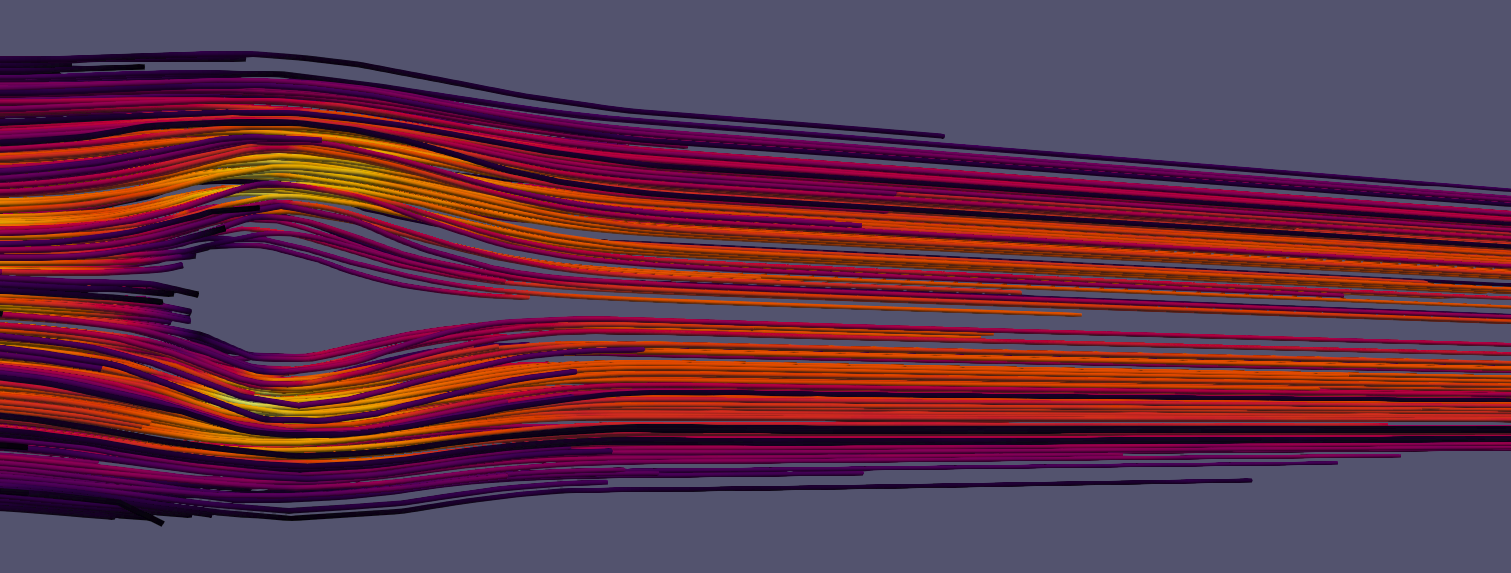
\includegraphics[width=\linewidth]{image/3d-arrows-20.png}\hfill
  \end{minipage}%
  \par
%   \begin{minipage}{\linewidth}
%   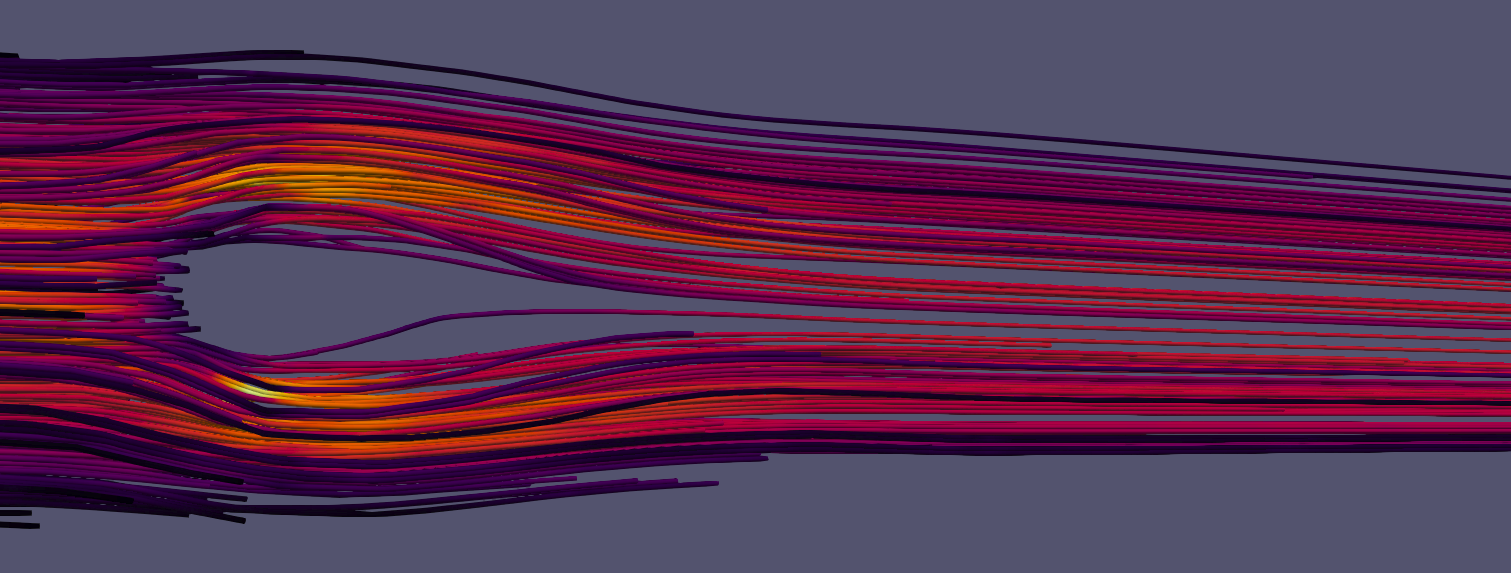
\includegraphics[width=\linewidth]{image/3d-arrows-48.png}\hfill
%   \end{minipage}%
%   \par
%   \begin{minipage}{\linewidth}
%   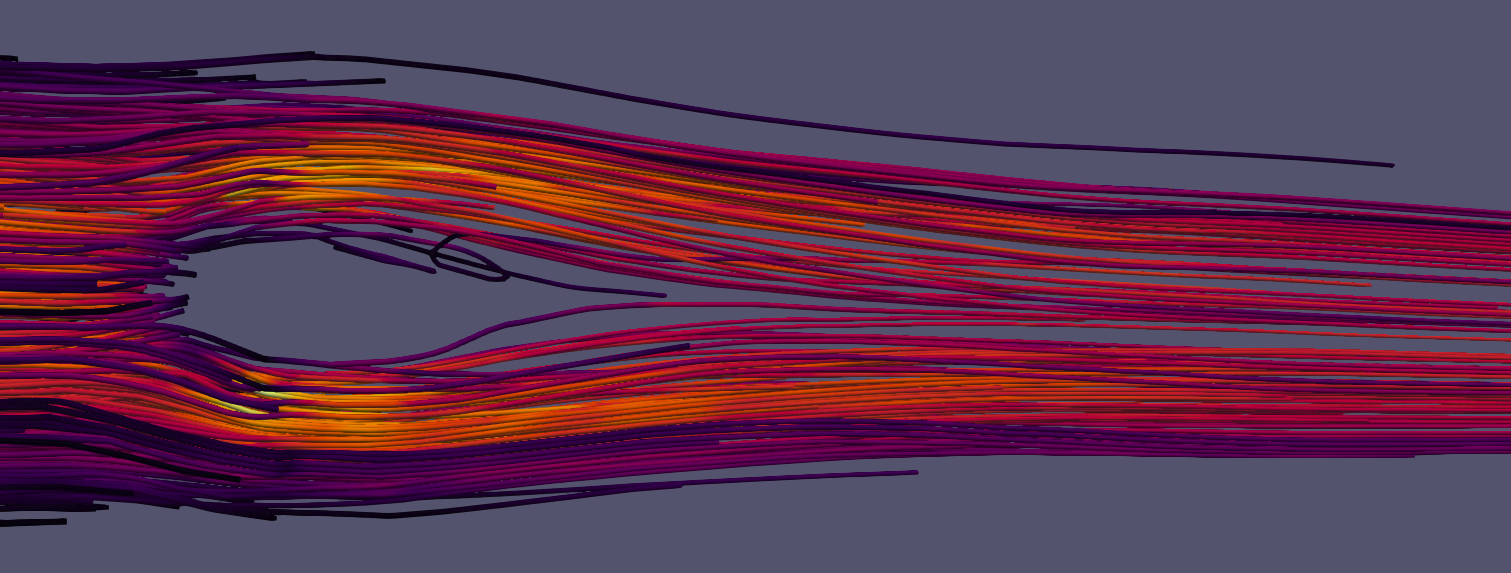
\includegraphics[width=\linewidth]{image/3d-arrows-100.png}\hfill
%   \end{minipage}%
%   \par
  \begin{minipage}{\linewidth}
  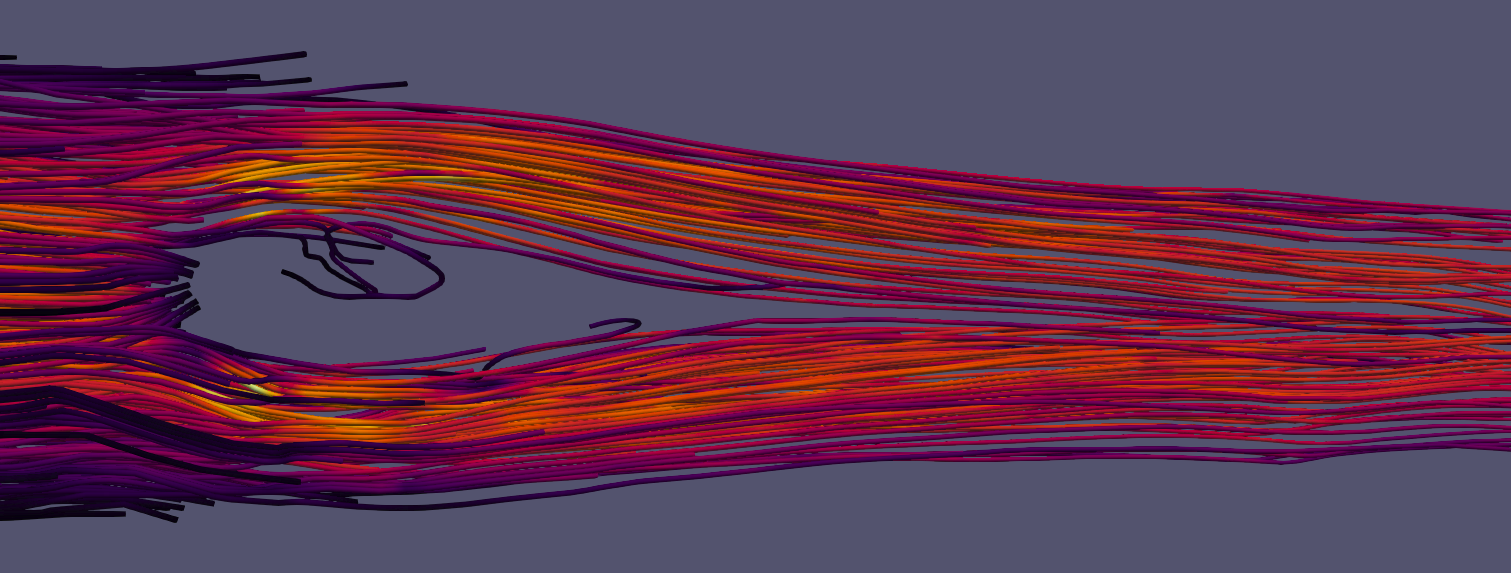
\includegraphics[width=\linewidth]{image/3d-arrows-200.png}\hfill
  \end{minipage}%
  
  \caption{Velocity stream lines at low and high Reynolds numbers, in 3D. The results were obtained with $\Delta t = 10^{-3}s$, on a mesh generated with the argument \texttt{-clmax 0.5} and are relative to $t = 1.5s$.}
  \label{fig:velocity-3d}
\end{figure}

\subsubsection{Results discussion}
A clear pattern can be seen in the velocity field, with the flow being laminar for low values of the Reynolds number and turbulent for higher values. This is consistent with the expected behavior of the flow, as vortex shedding is expected to occur for higher values of the Reynolds number. The pressure field is also consistent with the expected behavior, with the pressure being higher on the front of the cylinder and lower on the back.
The effects of vortex on lift and drag are also visible in section \ref{sec:lift_drag_plots}, where the lift and drag coefficients are plotted against time.